\chapter{Document Retrieval}
\label{chap:docret}

The term document retrieval refers to the task of finding relevant information to user queries in a large set of records (documents). 
% Therefore, the document retrieval system operates over a database of records, which for this thesis are described in \ref{chap:data}.
One can think of document retrieval as a search in a vast database of documents. 
In this view, web search services, such as Google, are also a form of document retrieval. 
In this case, the database of documents is all the accessible web pages on the internet.

For our uses, the query is the claim to be fact-checked, and the document database is a collection of relevant documents, which we call knowledge base. 

\section{Formal Description}
\label{sec:formal_descr_dr}
The task can be formally described \citep{two-tower} using a scoring function (sometimes referred to as ranking function) %article before ranking maybe
$$f_\mathcal{D}\colon\mathcal{D}\times\mathcal{Q}\rightarrow\R$$
that maps a document-query pair $(d, q)$ to a score $f(d,q)$. 
Then, typically, the documents in pairs with the highest scores are considered to be the proposed solution to the task. 

As mentioned above, this definition also fits descriptions of a range of other tasks such as open-domain question answering \citep{wiki-retrieval} or recommendation systems.

\section{Approaches to Document Retrieval}

The organizators of \textbf{T}ext \textbf{Re}trieval \textbf{C}onference (TREC) \citep{trec-2020} classify retrieval methods into three categories (with examples):
\begin{itemize}
        \item Traditional -- TFIDF, BM25
        \item Neural Networks using Language Modeling (NNLM) -- BERT-based
        \item Neural Networks -- others
\end{itemize}
We explore NNLM and traditional approaches, emphasizing the NNLM approach while using the other as the baseline. ``Neural Networks'' is reserved for methods that use neural networks only in some parts of its implementation (such as word embeddings) and do not rely explicitly on language modeling. We do not explore such methods in this thesis, and therefore, by neural approach, we refer to NNLM methods
While both work on entirely different principles, we will use both to generate an indexed version of the knowledge scope.

This chapter further introduces the most common document retrieval methods and new models with great potential while explaining the main points of the theoretical background.

\section{Traditional Approaches}

Traditional approaches covered are weighting schemes, assigning a query-dependent score to each word in each document in the database.

\subsection{TFIDF}

The traditional approaches are motivated by the intuition that relevant documents will contain the same words as those present in the query. 
Longer documents are at an advantage since there is a higher chance of the relevant words being present, so the term count is often normalized by the number of all terms in the document.
This simple metric is called term frequency (TF). 

TF can be ineffective if some of the terms in the query are very common in the document database.
This issue is resolved by introducing inverse document frequency, which informs how common the term is across all the documents.
The base version of IDF:
$$\text{idf}(t, D)=\log{\frac{\abs{D}}{\abs{\{d\in D: t\in d\}}}}\ .$$

% If we combine these two metrics
Multiplying these two metrics, we get the TFIDF weight of term $t$ in document $d$ in document database $D$:
%which is calculated simply as
$$\text{tfidf}(t,d,D)=\text{tf}(t,d)\cdot\text{idf}(t,D)\ .$$

\begin{figure}[!htb]
	\centering
	\begin{minipage}{.5\textwidth}
		\centering
		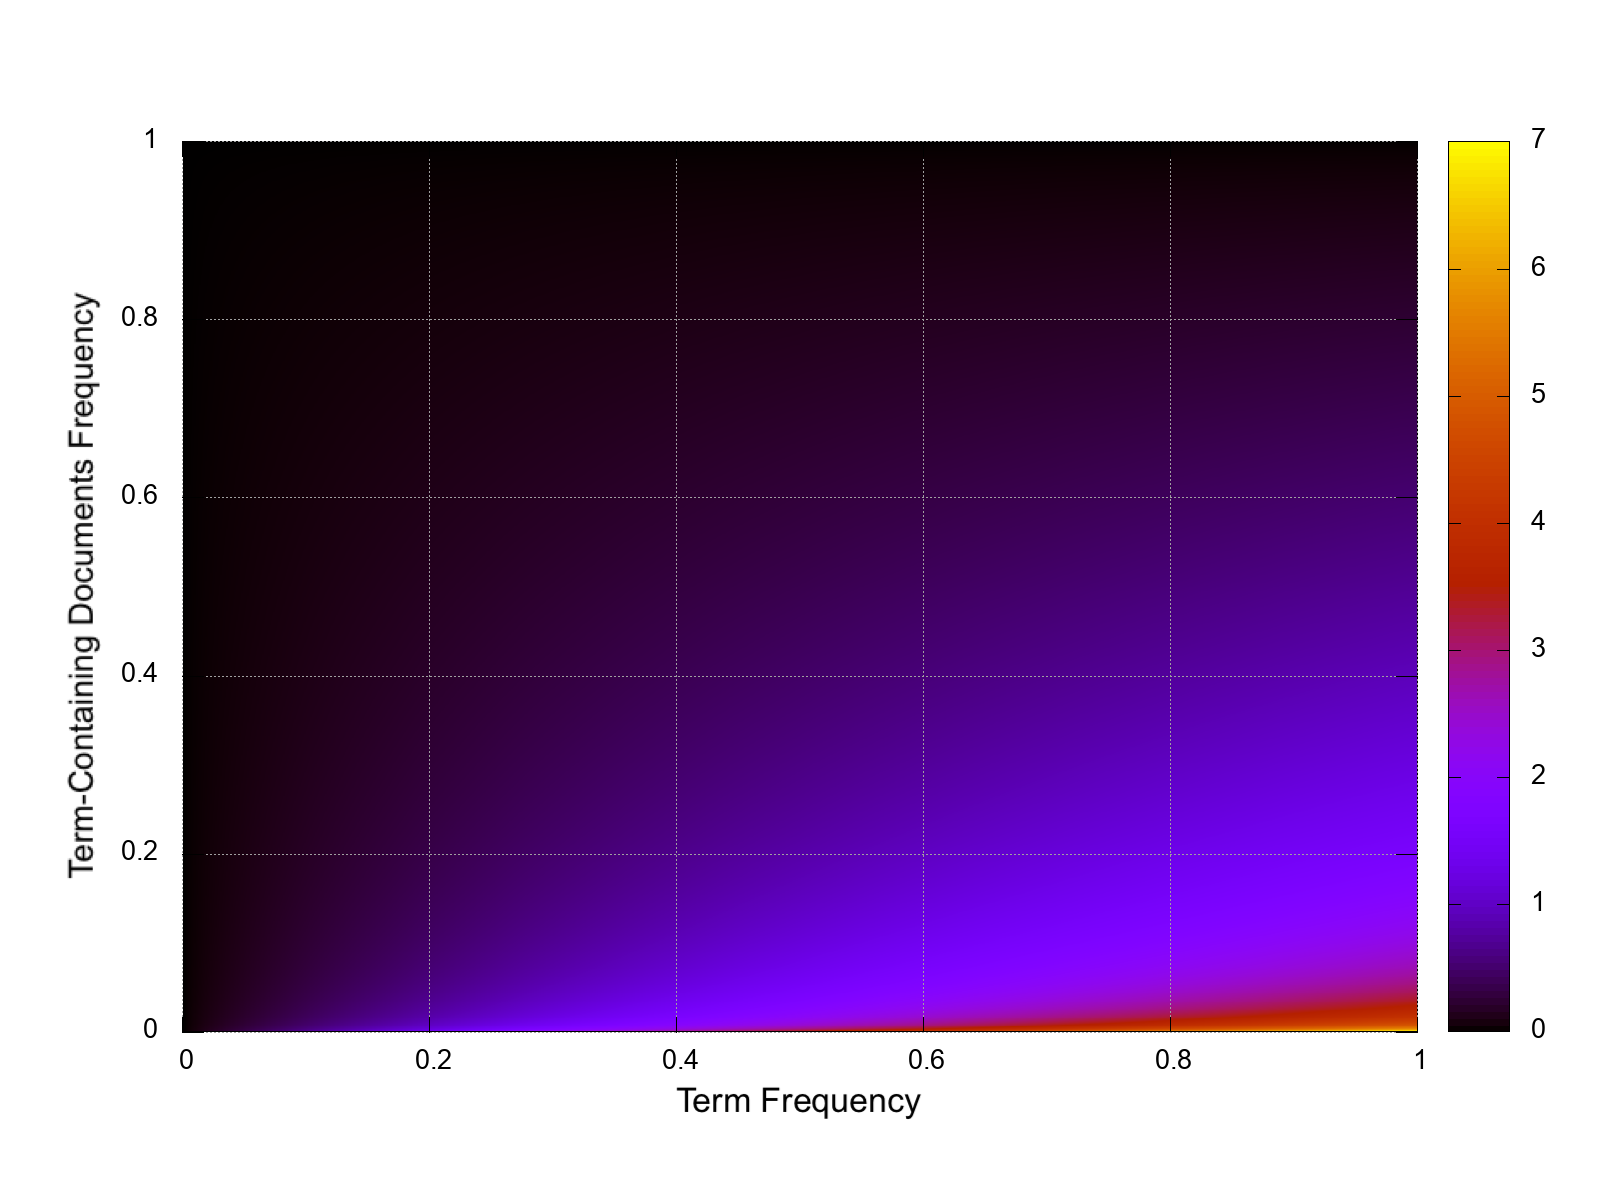
\includegraphics[width=\linewidth]{tfdif_map.png}
	\end{minipage}%
	\begin{minipage}{.5\textwidth}
		\centering
		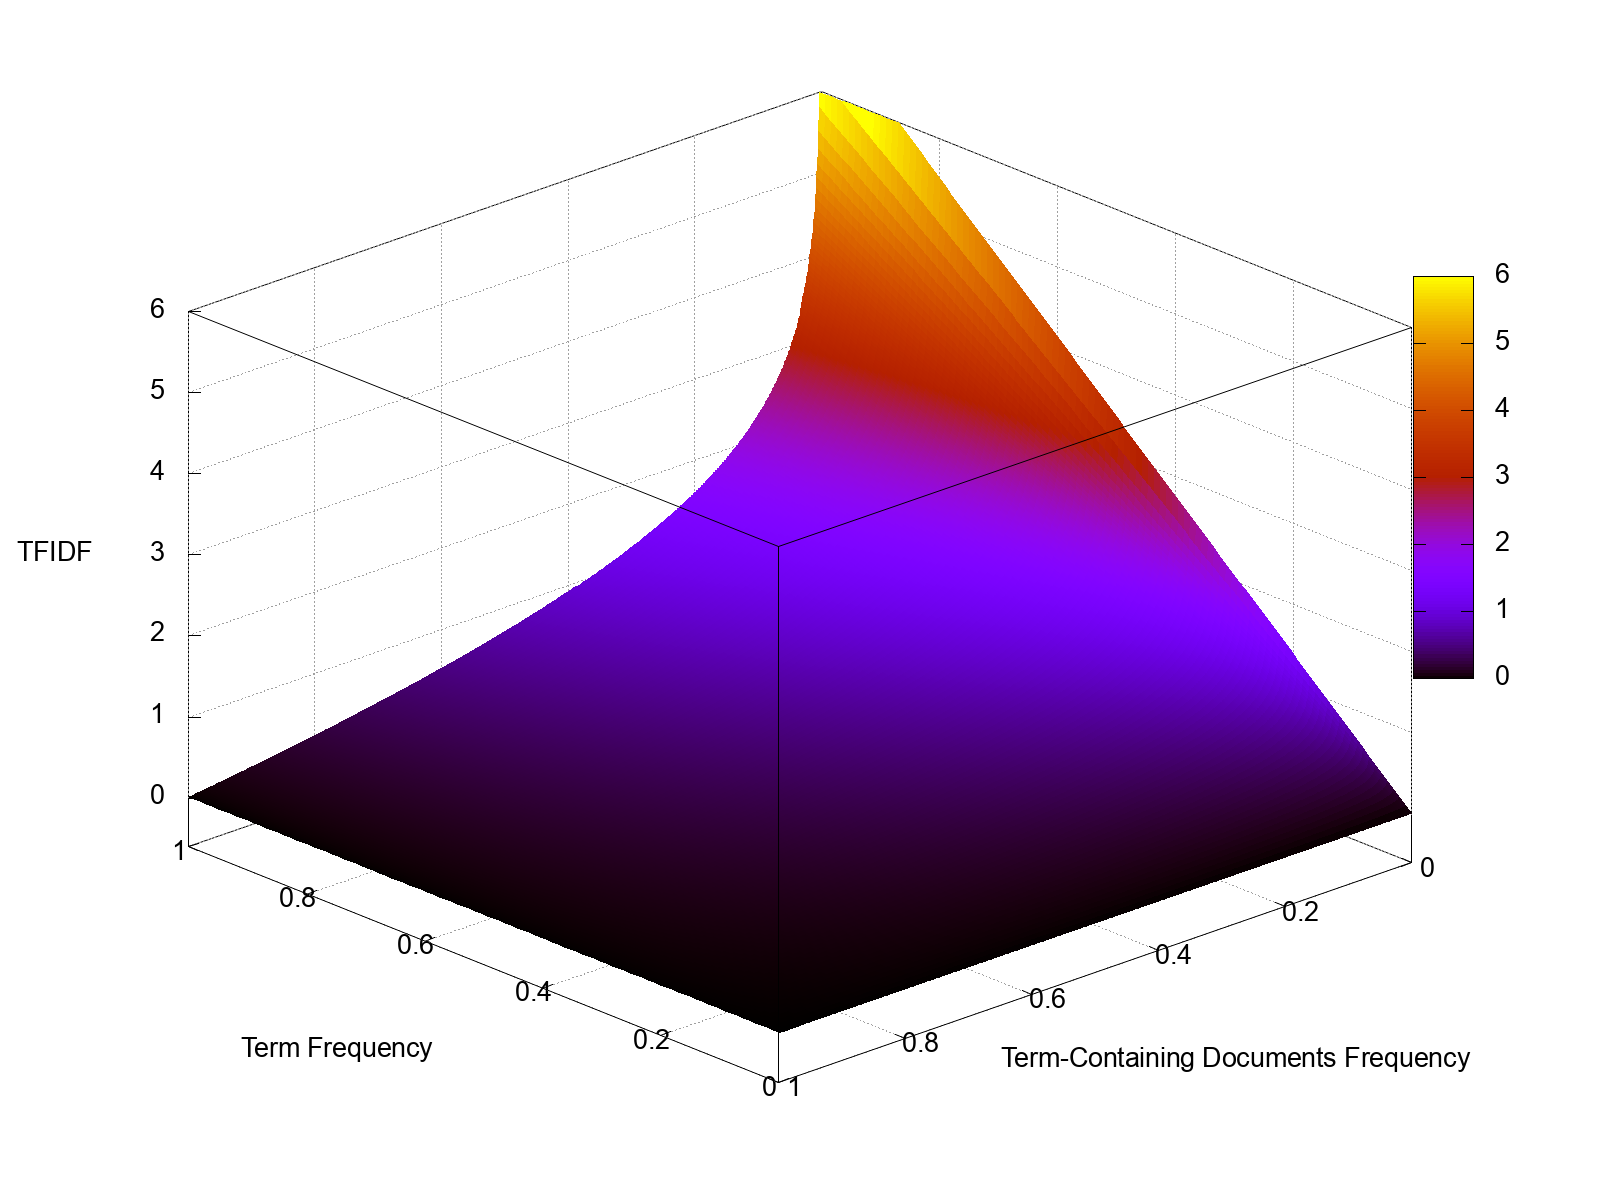
\includegraphics[width=\linewidth]{tfidf.png}
	\end{minipage}
        \caption{Visualization of TFIDF depending on the term frequency and the frequency of the documents containing the term.}
\end{figure}

We have explained how to compute a term's weight (``importance'') for a specific document.
The intuitive formula for query score $f(q, d)$ is then
$$
f_D(q, d)\approx\sum_{t \in q}\text{tfidf}(t, d, D)\ .
$$
TFIDF is called a weighting scheme precisely for this reason.

Since % term frequency and therefore tfidf is zero when 
$$t\notin d \hspace{1mm}\Rightarrow\hspace{1mm} \text{tf}(t, d) = 0 \hspace{1mm}\Rightarrow\hspace{1mm} \text{tfidf}(t, d, D) = 0\ ,$$
we know that only words in the corpus' vocabulary are important, and thus we can precompute the TFIDF values for each document, and word from the corpus' vocabulary.
We obtain $|D|\times {vocabulary\_size}$ matrix $V$ of TFIDF values.
%This formula can be improved -- in this form, it favors longer queries $q$. % DOES IT? TODO
%We can also precompute the TFIDF values for each document and vocabulary word in the corpus.
%Thus we obtain $|D|\times {vocabulary\_size}$ matrix $V$ of TFIDF values.
Here, to simplify length normalization, we normalize the matrix V so that each row has unit norm.
This step removes the need of normalization in the TFIDF formula and we may use raw term count instead of the normalized frequency.
To get the relevance of each document to the query $q$, that is $f_D(q, d)$, we first represent the query $q$ as a bag of words vector (BOW), corresponding to the columns of our precomputed TFIDF matrix $V$, ignoring words that appear only in the query.
The resulting score is then the normalized (not to favor long queries) dot product of a row of the matrix and the BOW representation of the query $q$ denoted $\vec{q}$.
We can obtain the scores for every query document pair by matrix multiplication:
$$
f_D(q, d) = \frac{V\vec{q}}{|\vec{q}|} \in \R^{|D|}\ ,
$$
provided that matrix $V$ is row-normalized (euclidian norm of each row is equal to one).
Please note that this is equivalent to computing the cosine similarity for each document and query vector pair.

This function is one of the first and still widely used \citep{Beel2016} weighting schemes for document retrieval. 

Over the years, multiple versions of the TFIDF approach appeared, differing slightly in formulas or weights of the factors. One of such versions is Best Match 25. %questionable TODO
% maybe put the last sentence as the last sentence of the whole section

\subsection{Best Match 25 (BM25)}

%The following is 
A more complex term weighting scheme is Best Match 25 \citep{bm25}:
%One of the best performing versions \citep{bm_vs_tfidf} is Best Match 25 (BM25) by \cite{bm25}.
%The original formula is:
$$
\text{BM25}(q, d) = 
        \sum_{t\in q}
        \text{idf}(t, d)
        \cdot \frac{(k_1 + 1)\cdot\text{count}(t, d)}{k_1(1-b + b \cdot (L_d / L_{avg})) + \text{count}(t, d)} 
        \cdot \frac{(k_3 + 1)\cdot\text{count}(t, q)}{k_3 + \text{count}(t, q)}
\ ,
$$
where $\text{count}(t,d)$ is the raw count of the term $t$ in the document $d$.

The first term is IDF.
The second term is TF with two tuning parameters $k_1$ and $b$. Parameter $k_1$ corresponds directly to TF scaling, while parameter $b$ corresponds to scaling by the inverse of the document's length.
The third term follows the same idea as the second term, but the $b$ parameter equivalent is unnecessary since we only have one fixed query.
It shows \citep{schutze2008introduction} that this term is only valid for longer queries $q$, such as whole paragraphs. 
\begin{figure}[h!]
    \centering
    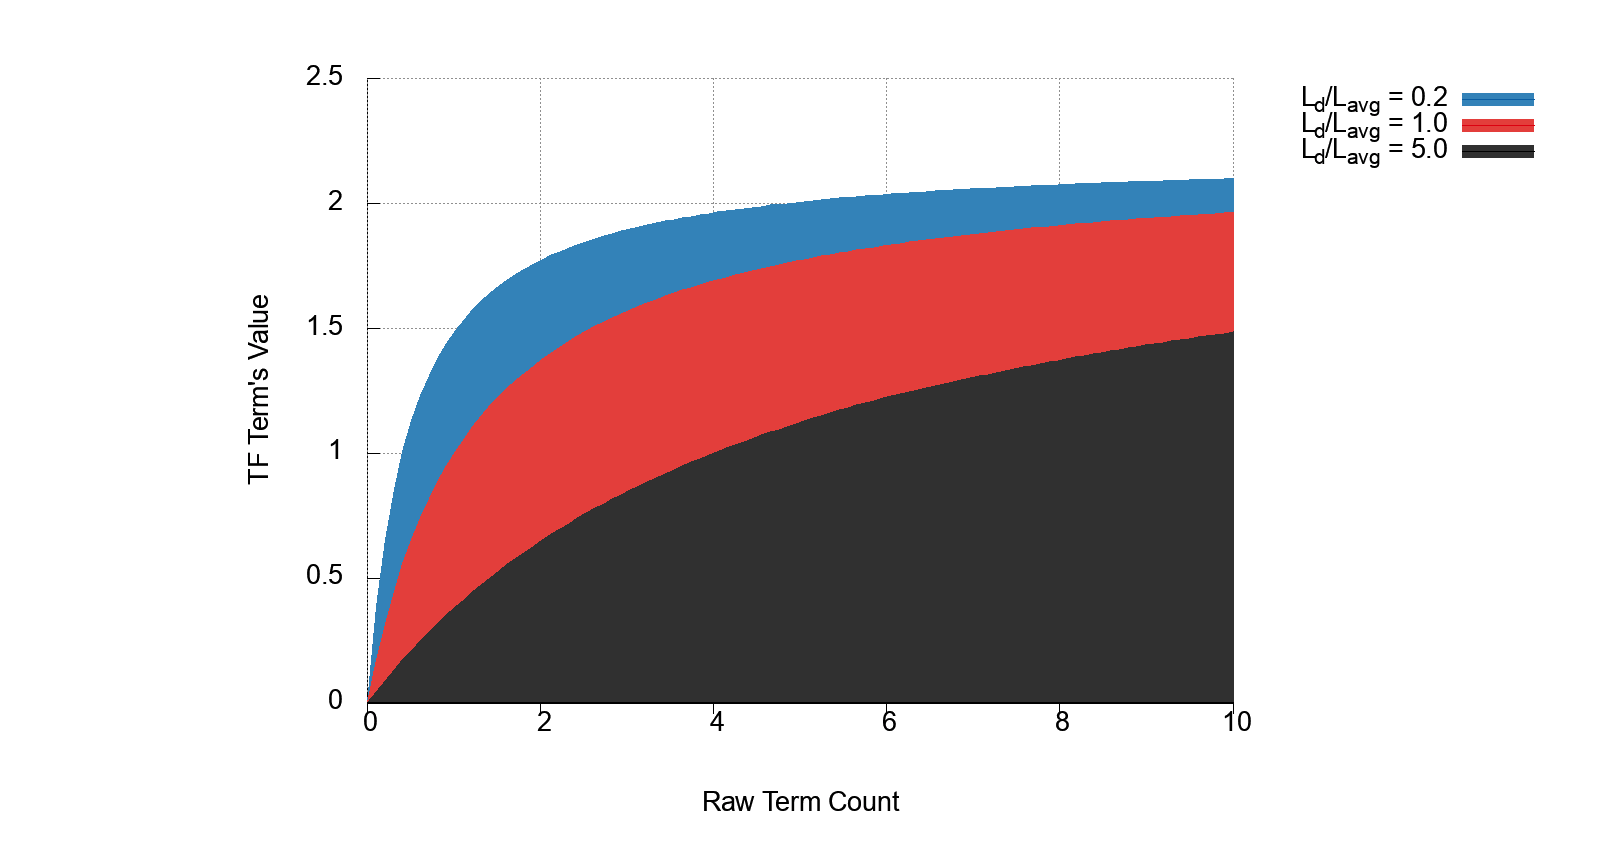
\includegraphics[width=.9\textwidth]{bm25.png}
    \caption{TF term's relation to the length of the current document for $k=1.2$ and $b=0.75$.}
\end{figure}

Since this weighting scheme introduces tunable parameters, it can be trained on data. If the data is not available, \citet[Section 11.4.3]{schutze2008introduction} recommend using $k_1, k_3 \in [1.2;2]$ and $b=0.75$.

%TODO problem with long documents - BM25+ http://sifaka.cs.uiuc.edu/~ylv2/pub/cikm11-lowerbound.pdf

\subsubsection{Final Thoughts}

Some of the apparent disadvantages of traditional approaches are the lack of semantic meaning that comes from the independence on the word order and the exact word matching. % independence???
The former may be improved by using n-grams and the latter using character-level features instead of words, especially in inflected languages such as Czech.
On the other hand, TFIDF is, to this day, a very well-performing low-computation cost ranking function, and as reported by \cite{weak-baselines}, BM25 (if tuned well) is still a solid baseline capable of beating even much more complex neural models.

\section{Neural Approaches}

Neural approaches using language modeling are models trained on predicting the correct word given some text before.  % maximizing the likelihood of correct word prediction in a text. 
% More precisely, it is a conditional language modeling since the prediction also depends on provided input.
Recurrent neural network (RNN) architecture was traditionally used for this task.
The RNN was fed encoded tokenized input, returning a hidden state which was next fed into the RNN again along the next input token.
% The RNN was fed encoded tokenized input, and the RNN predicted the next token as depicted in Figure \ref{fig:lec6_slide23}.
Its hidden states could also be used to encode the input into a fixed-length vector representation, which can be further used to either classify the input or use another RNN (decoder) to generate another sequence.
Intuitively, the vector contains the meaning of the original input. 
Such an approach is the Sequence to Sequence (seq2seq or encoder-decoder) model architecture \citep{seq2seq} with significant use-case in machine translation.

As an improvement to the seq2seq models, the attention mechanism was introduced by \citet{first-attention}, explaining their motivation as follows: ``In this paper, we conjecture that the use of a fixed-length vector is a bottleneck in improving the performance of this basic encoder-decoder architecture, and propose to extend this by allowing a model to automatically (soft-)search for parts of a source sentence that are relevant to predicting a target word, without having to form these parts as a hard segment explicitly.'' The attention mechanism is in-depth described in subsection \ref{subsec:attention}.

% TODO check if this sits nicely
\begin{figure}[b!]
        \centering
        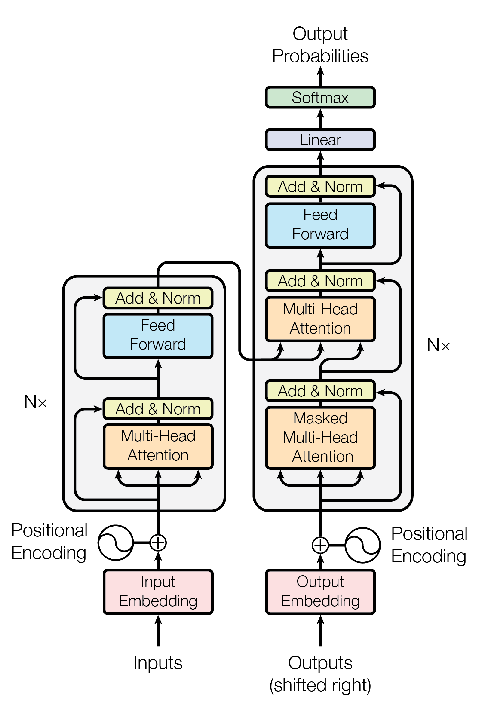
\includegraphics[width=.5\textwidth]{transformer.pdf}
        \caption{The transformer model architecture. Reprinted from \citep{attention-is-all-you-need}.}
        \label{fig:transformer}
\end{figure}

The research paper ``Attention Is All You Need'' by \citet{attention-is-all-you-need} improved the RNN-based seq2seq by introducing the transformer architecture, depicted in Figure \ref{fig:transformer}, by substituting the RNN by multiple ``encoder blocks'', that is, attention layer and feedforward network with skip-connection. 
This resulted in simpler architecture (RNN architectures tend to become very complex when trying to avoid the vanishing gradient problem), parallelization of the computation, and, most importantly, an improved performance. 
The improvement showed that the attention mechanism was crucial to the past achievements of the seq2seq models, hence the paper's name.
On the other hand, the attention mechanism also introduces quadratic time complexity, which is why the transformer models are generally used with fixed 512 token input length.
That might be adequate for most applications, but in document retrieval, the documents might get truncated. 
% neviem kam to quadratic TODO

Then \textbf{B}idirectional \textbf{E}ncoder \textbf{R}epresentations from \textbf{T}ransformers (BERT) \citep{bert} model was introduced. It was ``designed to pre-train deep bidirectional representations from unlabeled text by jointly conditioning on both left and right context in all layers''. 
The model can then be fine-tuned on a specific task using a small amount of labeled data and one additional output layer. 

This was a brief description of how a sequence of research papers -- ``Sequence to Sequence Learning with Neural Networks'' \citep{seq2seq}, ``Neural Machine Translation by Jointly Learning to Align and Translate'' \citep{first-attention}, ``Attention Is All You Need'' \citep{attention-is-all-you-need}, and ``BERT: Pre-training of Deep Bidirectional Transformers for Language Understanding'' \citep{bert} -- led to a shift from RNN-based NLP approaches to, now SOTA, BERT-based approaches.
This research focus is sometimes referred to as BERTology.

In the following sections, we will explain the concepts mentioned above in greater detail.

%The authors trained the model on a large unlabeled corpus using two tasks. 
%The first was to predict random masked words, and the second classified whether the second sentence of two selected sentences immediately follows the first one.
%It is a language modeling encoder capable of non-supervised learning 

\subsection{Attention Mechanism}
\label{subsec:attention}

The main feature of the transformer models is the attention mechanism. It adjusts each token's embedding based on all the other tokens present in the current input.
This is done by computing three different projections of the original input tokens and then, based on certain similarities, combining them back together. 
The attention mechanism is also reffered to as self-attention, since all the tokens in one input attend to the same input.

The projections are computed using trainable matrices $W_Q$, $W_K$, and $W_V$, producing queries $Q$, keys $K$, and values $V$. Then, we compute the dot product (``similarity'') between the keys and the queries $QK^T$, illustrated in Figure \ref{fig:self-attn}.
The result is normalized by the inverse factor of the square root of the projection dimension. 
Then softmax is applied, and the result is used as the weights for the weighted average of all value vectors. To put it into an equation: $$\text{softmax}(\frac{QK^T}{\sqrt{d}})V\ .$$
Therefore, for every token, the result is the weighted average of all the value vectors, based on the similarity between the queries and the keys. 
The result is called scaled dot-product attention.

\begin{figure}[!htb]
	\centering
	\begin{minipage}{.49\textwidth}
		\centering
		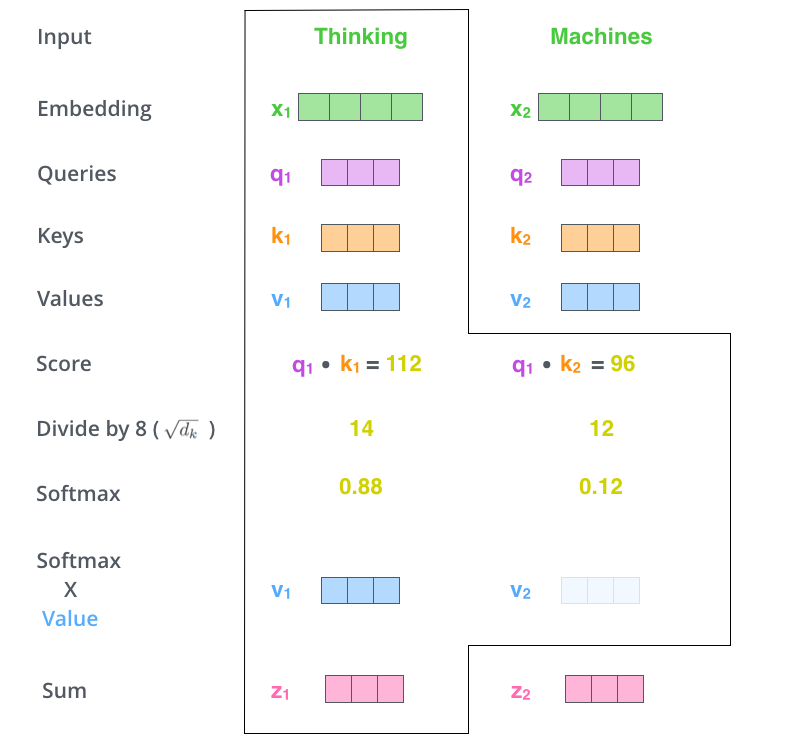
\includegraphics[width=\linewidth]{self_attention_output.png}
                \caption{Example of self attention mechanism with projection dimension 64 and the input ``Thinking Machines''. Reprinted from \citep{illustrated-transformer}.}
	\end{minipage}
        \hfill
	\begin{minipage}{.49\textwidth}
		\centering
		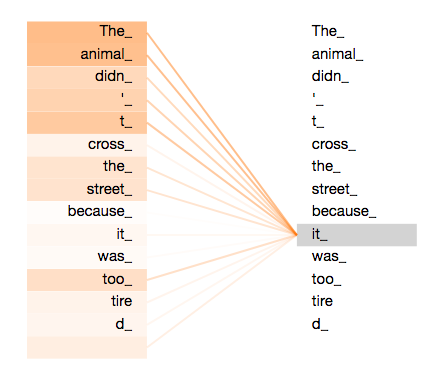
\includegraphics[width=\linewidth]{self_attention_visualization.png}
                \caption{Self-attention mechanism example, where the token for word ``it'' is paying attention to ``the animal'', effectively being substituted for it. The orange color represnts the values from $QK^T$. Reprinted from \citep{illustrated-transformer}.}
                \label{fig:self-attn}
	\end{minipage}
\end{figure}

The computation is performed multiple times in parallel with independent projection matrices to make the mechanism more robust.
The results are then concatenated and projected into the final dimensionality.
This extended attention is called multi-head attention.
The intuition is that different heads might learn to attend to different patterns and meaning subspaces.

\subsection{Transformers}

positional encoding

\subsection{BERTology}

\COMMENT{%%%%%%%%%%%%%%%%%%%%%%%%%%%%%%%%%%%%%%%%%%%%%%%%%%%%%%%%%%
Traditional approaches will result in sparse representation with the feature dimension size equal typically to the corpus's vocabulary size (the vocabulary can also contain n-grams or character n-grams if it is advantageous).
Therefore, it can be considered a weighting scheme, assigning "importance" to each word if it was present in the document. 
Neural approaches used in this paper produce a dense representation, as described by \citet{two-tower}.
It is usually a fixed-size vector of real numbers, inherently hard to interpret.
The meaning can be derived only from the relative position of different documents' indexes (vectors).

Neural models can also be used directly as the scoring function as in Section \ref{sec:formal_descr_dr}.
This can, according to \citet{two-tower}, lead to better performance. However, since the query is provided at runtime, the evaluation cannot be precomputed and has to run for every document each time we enter a new query.
This is currently infeasible for usage on whole corpora but can be utilized by running on a smaller subset of the corpus (so-called reranking), typically pre-selected by a non-neural model, creating a hybrid approach.

% TODO two-tower paper, 
In order to solve the document retrieval task, we will focus on finding an appropriate function $f$.
In this thesis, that means a function suitable for long documents.
}

As mentioned above, when dealing with natural language processing, we can approach the task in two different ways, both described in detail by \cite{two-tower}. 

The first is to have the document-query pair $(d,q)$ on the input of the neural model (cross-attention model).
One of the benefits is the direct usage of the neural model on the downstream tasks, possibly granting better performance.

The second approach is to preprocess the whole database of documents by the model and then using some metric for choosing the documents related to the query based on the computed representation.
The obvious advantage is the offline preprocessing and thus improved performance during inference.
Only the unseen query has to be processed by the neural model followed by computing the metric between the documents' representation and the query representation.
This is usually way faster than using a neural model for every document and can also be significantly spedup \citep{faiss}.
The obvious disadvantage is the need for additional space to store the precomputed representation.

We will be using the second approach as our computational resources are limited.

% TODO under this line ---------------------------------
\subsection{BERT}
In 2018, BERT \citep{bert} the now well-established NLP model was introduced. The model is pre-trained using the masked language modeling task and the next sentence prediction task.
The defining feature of BERT is its self-attention mechanism, which attends to the whole input at once and transforms input tokens based on full context, both left, and right to the token.
Since the "each versus each" approach is employed, this mechanism naturally introduces $O(N^2)$ time complexity, which acts as a bottleneck in applications, where a longer input is required.
Since its introduction, there have been many well-performing models based on BERT (this movement is sometimes referred to as "BERTology").
In this thesis, we will focus on models which use similar architecture and modify attention mechanism in order to be able to compute long inputs.
% used usually for GLUE benchmark which is not???? for document retrieval
% TODO maybe include attention formula

\subsection{Longformer}

Longformer model \citep{longformer} arises when instead of computing the whole $QK^T$, only certain regions (usually specific diagonals) are calculated, thus reducing the model time complexity allowing for longer inputs.
Huggingface models are available.

\subsection{Reformer}

Reformer model \citep{reformer} offers two improvements to the transformer model.
The first is the usage of locality-sensitive hashing in the attention mechanism, which in order to approximate the full attention matrix focuses for each input token only on the closest tokens.
The closest tokens are found using the locality-sensitive hashing function.
This, coupled with memory saving features, offers a model which can have a whole novel as its single input.

\subsection{Performer}

Performer model \citep{performer} looks at the self-attention mechanism as a kernel function and introduces randomized feature functions such that the expected value of scalar product %????%e
of the resulting feature vectors is equal to the true value.
% TODO weak ensurences

\subsection{\nystr{}}

\nystr{} \citep{nystrom} uses ``smart'' Moore-Penrose inverse approximation. Instead of full $Q$ and $K$ matrices, only segment-means are used, and then the Moore-Penrose inverse is calculated using an iterative algorithm.

\subsection{ColBERT}

\citep{colbert}
TODO Martinove výsledky cite


